\section{监督来源、集成与诊断对照}\label{sec:controls}

\subsection{融合监督与分支监督}
\label{sec:source-ablation}
固定 J 时，F、T 和 G 的平均增益分别为 $+0.155665$、$+0.134868$ 和 $+0.040991$。F 相对 T 的优势为 $+0.020797\pm0.001214$，相对 G 的优势为 $+0.114674\pm0.001001$，两组差异在全部三个种子上均为正。融合组成与预测质量同时发生变化，因此该对照不能单独确定融合收益的来源。

仅使用 T 的监督条件在资格门控阶段和首个正式训练轮次中，每次更新都会触发梯度裁剪，尽管参数梯度均为有限值。获准继续进行的续训保留了 \texttt{CLIP\_SATURATION\_WARNING}。应谨慎解释较小的 F--T 差距；附录~\ref{app:protocols} 记录了保持不变的训练协议与裁剪轨迹。

\subsection{同构集成证伪对照}
\label{sec:homogeneous-control}
TT 的增益为 $+0.168125\pm0.008948$，TG 的增益为 $+0.155665\pm0.007692$。配对差异定义为
\begin{equation}
H=\mathrm{Gain}_{\mathrm{TG}}-\mathrm{Gain}_{\mathrm{TT}}
=\mathrm{NLL}_{\mathrm{TT}}-\mathrm{NLL}_{\mathrm{TG}},
\label{eq:ensemble-contrast}
\end{equation}
其均值为 $-0.012460\pm0.001348$，全部三个差异均为负。在所测试的设置中，TG 教师模型相较于 TT 没有优势（图~\ref{fig:ensemble_control}）。

TT 教师模型在完整验证集上的 NLL 还低 0.010108，参数量约少 6.38\%，且融合权重学习率与训练历程均不同。这些混杂因素使得该排序不能归因于 TT 的内在优势。TG 的分支分歧更大，但 KD 增益并未更大；预测多样性不一定是可迁移的多样性。该比较不支持 Grassmann 特有优势或异构监督优势。

\subsection{局部诊断指标不能区分最终结果}
\label{sec:local-diagnostics}
在七个教师模型--领域组合、每个组合三个学生种子的回顾性分析中，一阶与二阶评分的 AUROC 均约为 0.644，符号准确率均约为 0.571。曲率没有增加符号区分能力，且这些评分将已知具有正向结果的 WikiText-2 组合判错。所测试的局部诊断指标不能可靠地预测这些最终结果。

一些标量预测指标对合并结果的区分能力更强，但这一规模较小且存在依赖关系的结果集合不能确立一般性的选择规则。在 CE 难度之外，词元级分支 JSD 增加的信息很少。附录~\ref{app:diagnostics-modern} 报告了完整指标、校准不稳定性及观察性分析的局限。这些失败涉及所测试的离线评分，不能推广到一般的自适应 KD 方法。

\begin{figure}[!t]
\centering
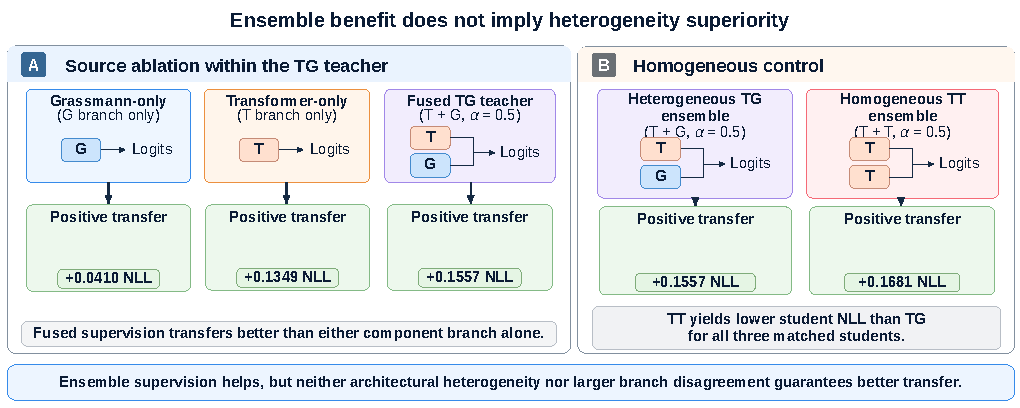
\includegraphics[width=\textwidth]{figures/fig4_ensemble_control.pdf}
\caption{WikiText-2 教师监督来源与集成的增益，保留四位小数。TT 在全部三个学生上均优于 TG。仅使用 T 的监督条件：早期裁剪饱和，应谨慎解释 F--T 差距。TT 与 TG 教师模型并非严格的质量匹配或训练匹配对照。}
\label{fig:ensemble_control}
\end{figure}
